\documentclass[a4paper,12pt]{article}
\usepackage{amsmath,amssymb,amsfonts,amsthm}
\usepackage{tikz}
\usepackage [utf8x] {inputenc}
\usepackage [T2A] {fontenc} 
\usepackage[russian]{babel}
\usepackage{cmap} 

% Так ссылки в PDF будут активны
\usepackage[unicode]{hyperref}

% вы сможете вставлять картинки командой \includegraphics[width=0.7\textwidth]{ИМЯ ФАЙЛА}
% получается подключать, как минимум, файлы .pdf, .jpg, .png.
\usepackage{graphicx}
% Если вы хотите явно указать поля:
\usepackage[margin=1in]{geometry}
% Или если вы хотите задать поля менее явно (чем больше DIV, тем больше места под текст):
% \usepackage[DIV=10]{typearea}

\usepackage{fancyhdr}

\newcommand{\bbR}{\mathbb R}%теперь вместо длинной команды \mathbb R (множество вещественных чисел) можно писать короткую запись \bbR. Вместо \bbR вы можете вписать любую строчку букв, которая начинается с '\'.
\newcommand{\eps}{\varepsilon}
\newcommand{\bbN}{\mathbb N}
\newcommand{\dif}{\mathrm{d}}

\newtheorem{Def}{Определение}


\pagestyle{fancy}
\makeatletter % сделать "@" "буквой", а не "спецсимволом" - можно использовать "служебные" команды, содержащие @ в названии
\fancyhead[L]{\footnotesize Термодинамика и молекулярная физика}%Это будет написано вверху страницы слева
\fancyhead[R]{\footnotesize ФМХФ МФТИ}
\fancyfoot[L]{\footnotesize \@author}%имя автора будет написано внизу страницы слева
\fancyfoot[R]{\thepage}%номер страницы —- внизу справа
\fancyfoot[C]{}%по центру внизу страницы пусто

\renewcommand{\maketitle}{%
	\noindent{\bfseries\scshape\large\@title\ \mdseries\upshape}\par
	\noindent {\large\itshape\@author}
	\vskip 2ex}
\makeatother
\def\dd#1#2{\frac{\partial#1}{\partial#2}}


\title{2.2.1 \\ Исследование взаимной диффузии газов} 
\author{Егор Берсенев} 
\date{27 февраля 2016 г.}

\begin{document}
	\maketitle
	\section{Цель работы}
		\begin{enumerate}
			\item Регистрация зависимости концентрации гелия в воздухе от времени с помощью датчиков теплопроводности при разных начальных давлениях смеси газов.
			\item Определение коэффициента диффузии по результатам измерений.
		\end{enumerate}
	\section{Оборудование}
		Измерительная установка, форвакуумный насос, баллон с гелием, манометр, источник питания, секундомер, мультиметр.
	\section{Теоретическая часть}
		\begin{Def}
			Диффузия --- самопроизвольное перемешивание молекул, происходящее вследствие их хаотичного теплового движения.
		\end{Def}
		В системе, состоящей из двух компонентов: $a$ и $b$, плотность потока вещества любого компонента определяется законом Фика:
		\begin{equation}
			j_a = -D_{ab}\dd{n_a}{x}, \quad j_b = -D_{ba}\dd{n_b}{x}
		\end{equation}
		где $D_{ab}=D_{ba}=D$ --- коэффициент взаимной диффузии компонентов, а $j_a, j_b$ --- плотности потока частиц.
		Можно предположить, что концентрация воздуха в условиях опыта много больше концетрации примеси гелия, поэтому относительное её изменение в результате взаимной диффузии будет незначительным. Поэтому будем описывать только диффузию примеси гелия на стационарном фоне воздуха, и под концентрацией $n$ будем понимать $n_{He}$. 
		\subsection{Устройство установки}
		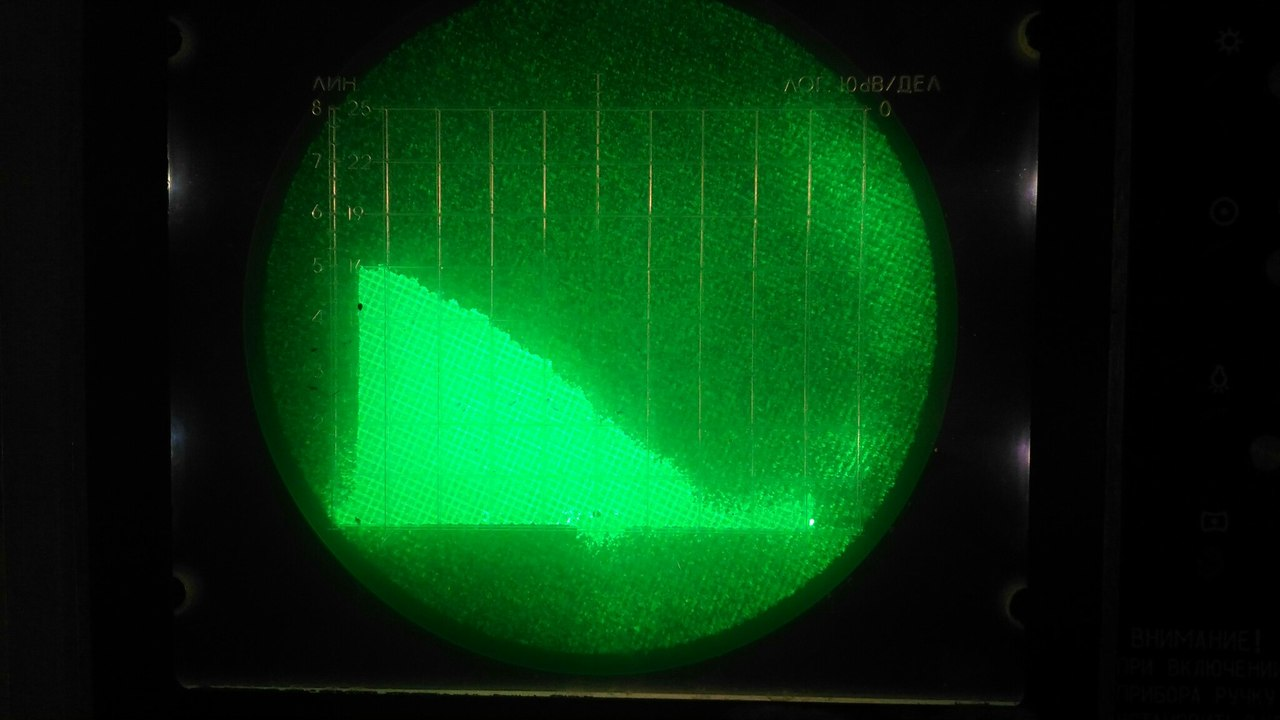
\includegraphics[width=0.5\textwidth]{pic1}
		
		Где:\begin{enumerate}
				\item Ф.Н --- форвакуумный насос;
				\item Т --- выключатель;
				\item П.Б --- предохранительный баллон;
				\item V --- сосуды;
				\item М --- манометр;
				\item D --- датчики теплопроводности.
			\end{enumerate}
		Концентрацию газов внутри каждого сосуда можно считать постоянной по всему объему сосуда, и предположить, что процесс выравнивания концетраций происходит в основном из-за диффузии в трубке.
		Если бы концентрации в сосудах поддерживались постоянными и равными $n_1$ и $n_2$, то в трубке бы установился стационарный поток частиц $J = -DS\dd{n}{x}$, одинаковый в каждом сечении трубки. Следовательно:
		\begin{equation}
			J = -DS\frac{n_1-n_2}{l}.
		\end{equation}
		В квазистатическом приближении найдем:
		\begin{equation}
			V_1\Delta n_1 = -V_2\Delta n_2 = J\Delta t = -DS\frac{n_1-n_2}{l}\Delta t
		\end{equation}
		\begin{equation}
			V_1\frac{\dif n_1}{\dif t} = -DS\frac{n_1-n_2}{l}, \quad V_2\frac{\dif n_2}{\dif t} = DS\frac{n_1-n_2}{l}.
		\end{equation}
		\begin{equation}
			\frac{\dif n_1}{\dif t}-\frac{\dif n_2}{\dif t} = -DS\frac{n_1-n_2}{l}\left(\frac{1}{V_1}+\frac{1}{V_2}\right).
		\end{equation}
		\begin{equation}
			\Delta n = \Delta n_0 e^{\frac{-t}{\tau}}
		\end{equation}
		\begin{equation}
			\tau = \frac{V_1V_2}{V_1+V_2}\frac{l}{DS}
		\end{equation}
	\section{Ход работы}
		\subsection{Параметры установки}
		\[ 
		V_1 = V_2 = 775 \pm 10\text{см}^3=\left(0.775\pm 0.001 \right)\cdot10^{-3}\,\text{м}^3 \qquad \frac{L}{S} = \left(5.3\pm 0.1\right)\cdot 10^{-2}\,\frac{1}{\text{м}} = 
		\]
		Тогда константа установки:
		\[
		c = \frac{V_1V_2}{V_1+V_2}\frac{L}{S} = 0.2 \pm 0.002 \,\text{м}^2
		\]
		\subsection{Измерения}
		\begin{center}
			\begin{tabular}{  l  l  p{1cm} |   l  l  p{1cm} |   l  l  p{1cm} }
				\multicolumn{9}{c}{\,P = 40 торр \qquad|\quad\qquad P = 120 торр \qquad\quad|\qquad P = 200 торр } \\ 
				Время, с & U, mV & ln U & Время, с & U, mV & ln U & Время, с & U, mV & ln U \\ \hline
				0   & 7.55  &  2.02 & 0   & 5.91  &  1.78 & 0   & 5.325  &  1.67 \\ \hline
				10  & 7.16  &  1.97 & 10  & 5.75  &  1.75 & 10  & 5.14  &  1.64 \\ \hline
				20  & 6.68  &  1.90 & 20  & 5.57  &  1.72 & 20  & 5.01  &  1.61 \\ \hline
				30  & 6.24  &  1.83 & 30  & 5.38  &  1.68 & 30  & 4.88  &  1.59 \\ \hline
				40  & 5.83  &  1.76 & 40  & 5.2   &  1.65 & 40  & 4.8  &  1.57 \\ \hline
				50  & 5.43  &  1.69 & 50  & 5.01  &  1.61 & 50  & 4.66  &  1.54 \\ \hline
				60  & 5.05  &  1.62 & 60  & 4.83  &  1.57 & 60  & 4.56  &  1.52 \\ \hline
				70  & 4.66  &  1.54 & 70  & 4.66  &  1.54 & 70  & 4.41  &  1.48 \\ \hline
				80  & 4.33  &  1.47 & 80  & 4.5   &  1.50 & 80  & 4.3  &  1.46 \\ \hline
				90  & 4     &  1.39 & 90  & 4.39  &  1.48 & 90  & 4.2    &  1.44 \\ \hline
				100 & 3.7   &  1.31 & 100 & 4.21  &  1.44 & 100 & 4.1   &  1.41 \\
				\hline
			\end{tabular}
		\end{center}
		\begin{center}
			\begin{tabular}{  l  l  p{1cm} | l  l  p{1cm}}
				\multicolumn{6}{c}{P = 280 торр\qquad |\qquad P = 360 торр} \\
				Время, с & U, mV & ln U & Время, с & U, mV & ln U \\ \hline
				0    & 2.5  &  0.92 & 0   & 2.7  &  0.99 \\ \hline
				10   & 2.42  &  0.88 & 10   & 2.66  &  0.98 \\ \hline
				20   & 2.36  &  0.86 & 20   & 2.66  &  0.98 \\ \hline
				30   & 2.29  &  0.83 & 30   & 2.57  &  0.94 \\ \hline
				40   & 2.21  &  0.79 & 40   & 2.52  &  0.92 \\ \hline
				50   & 2.15  &  0.77 & 50   & 2.47  &  0.90 \\ \hline
				60   & 2.08  &  0.73 & 60   & 2.42  &  0.88 \\ \hline
				70   & 2.02  &  0.7 & 70   & 2.37  &  0.86 \\ \hline
				80   & 1.97  &  0.68 & 80   & 2.33  &  0.85 \\ \hline
				90   & 1.91  &  0.65 & 90   & 2.28  &  0.82 \\ \hline
				100   & 1.87  &  0.63 & 100   & 2.24  &  0.81 \\ \hline
			\end{tabular}
		\end{center}
		\subsection{Обработка результатов}
		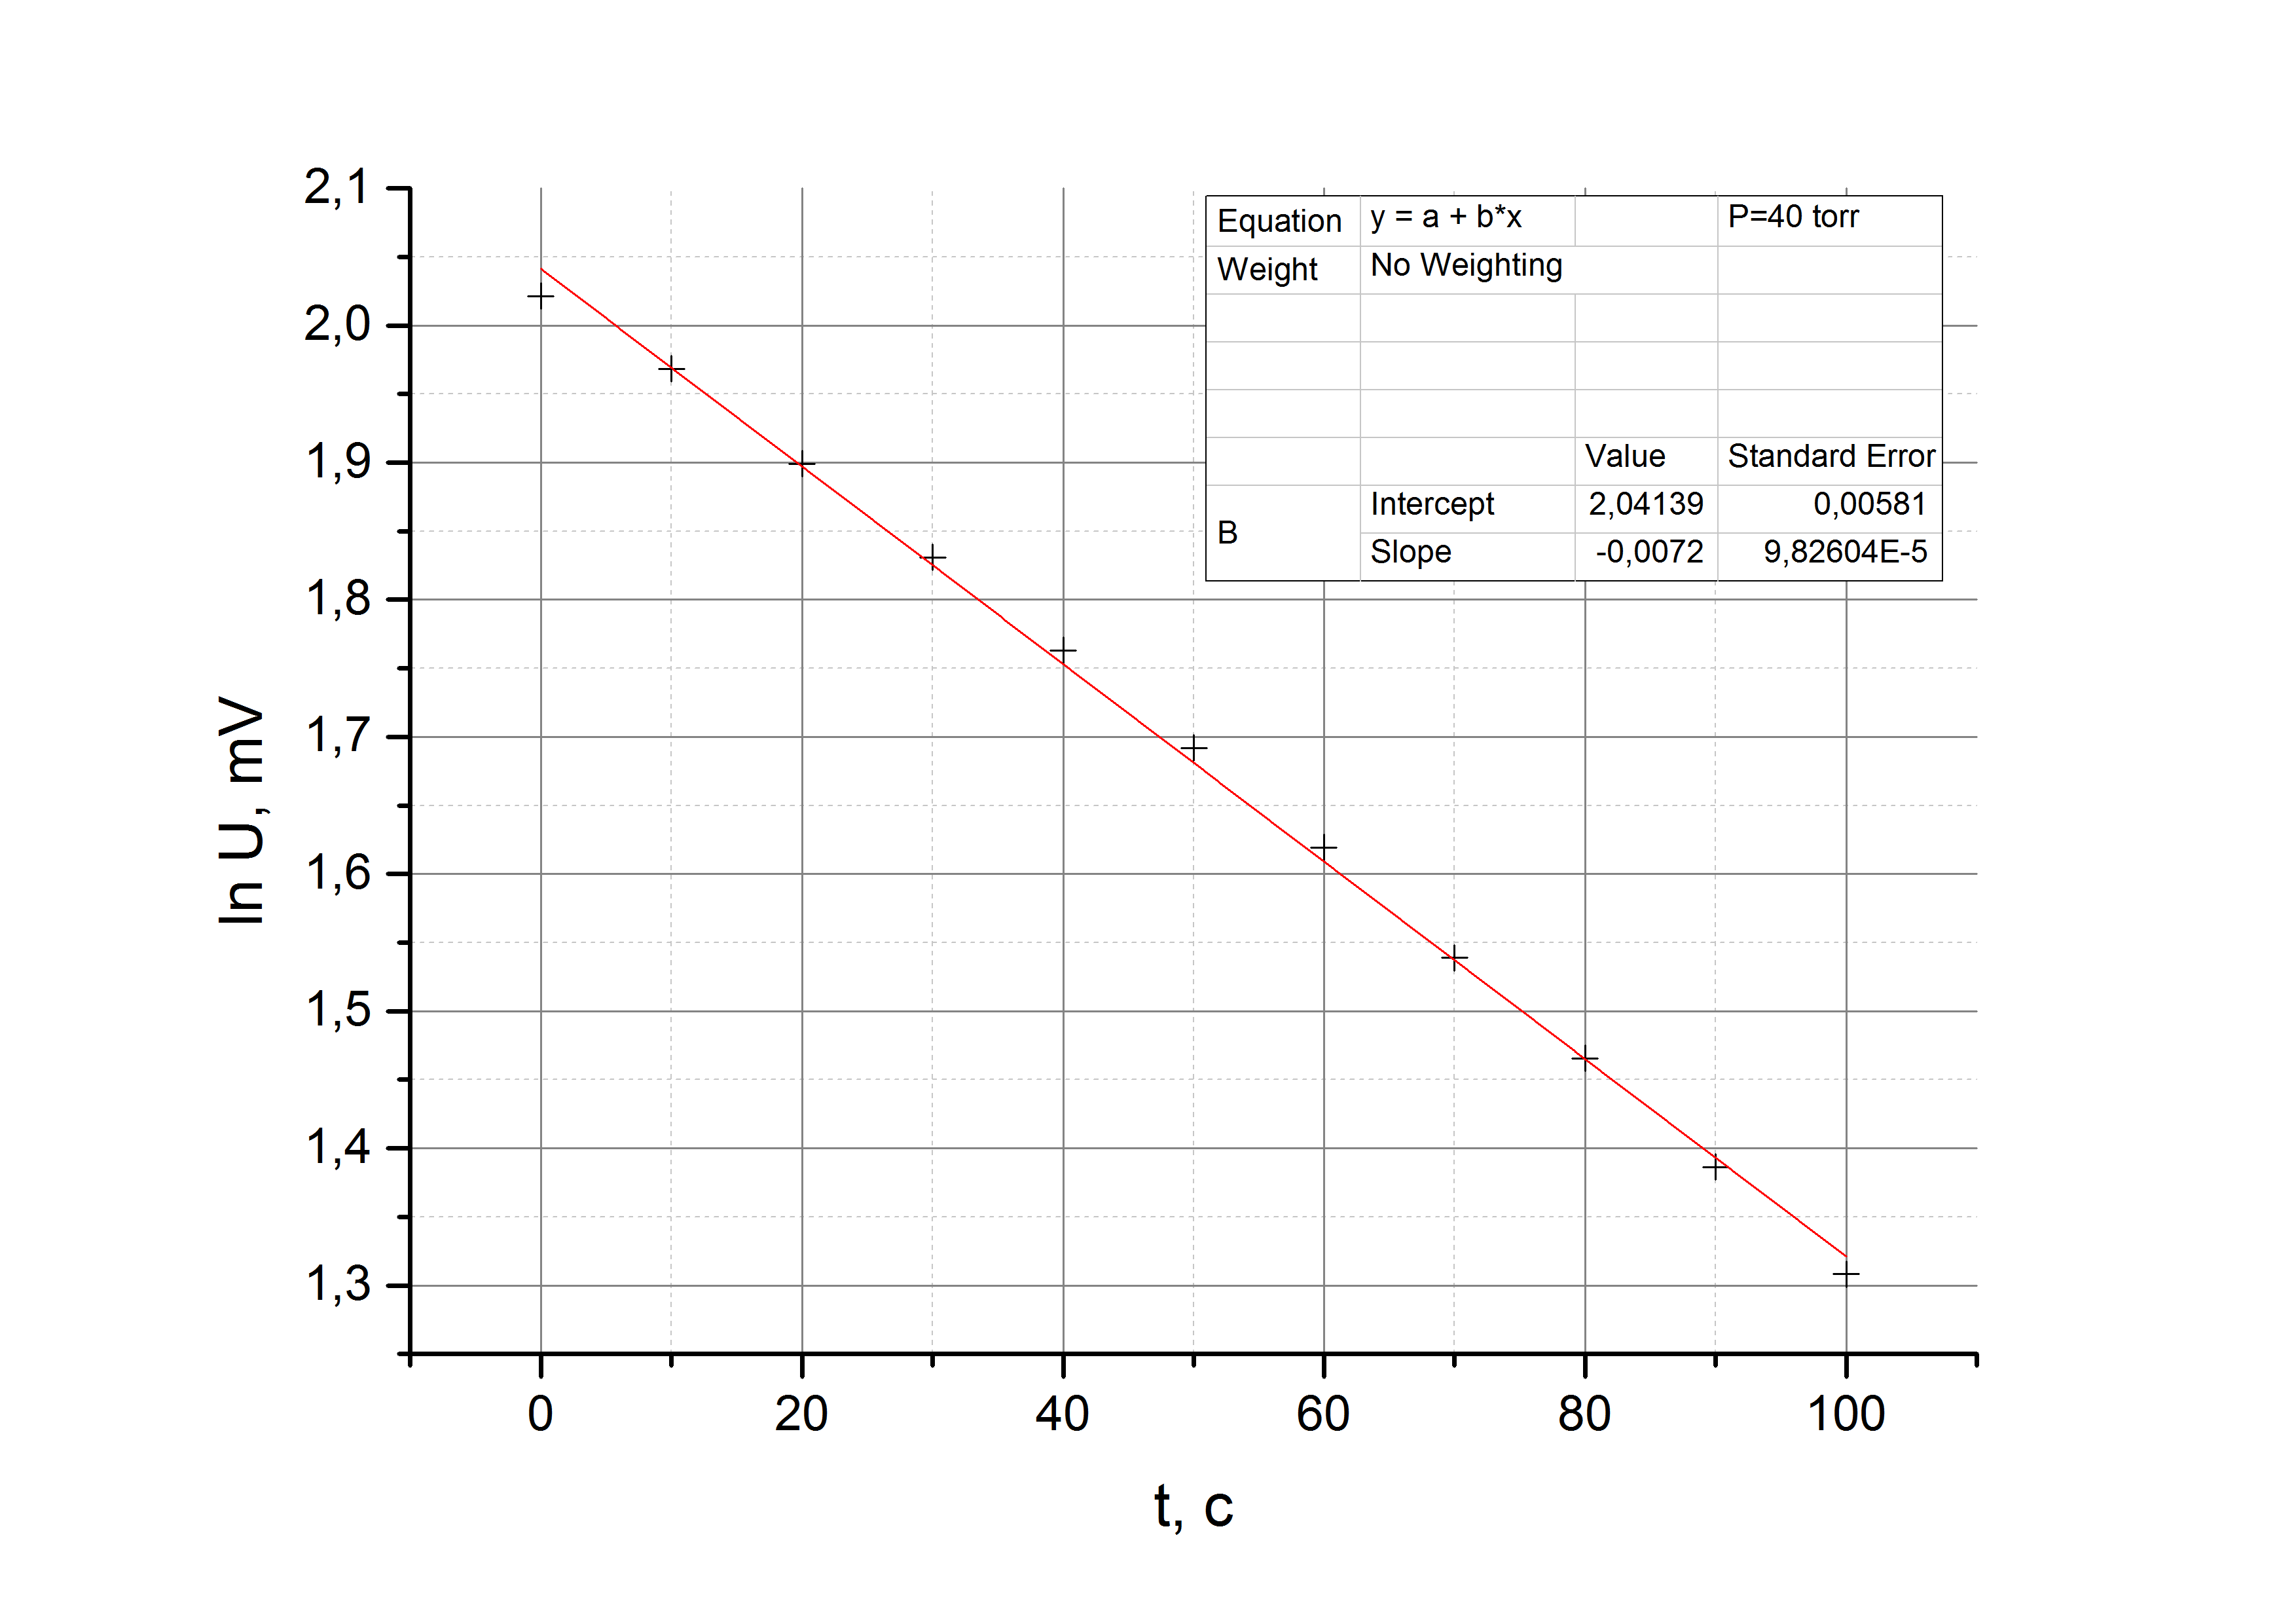
\includegraphics[width = 0.75\linewidth]{40torr}\newline
		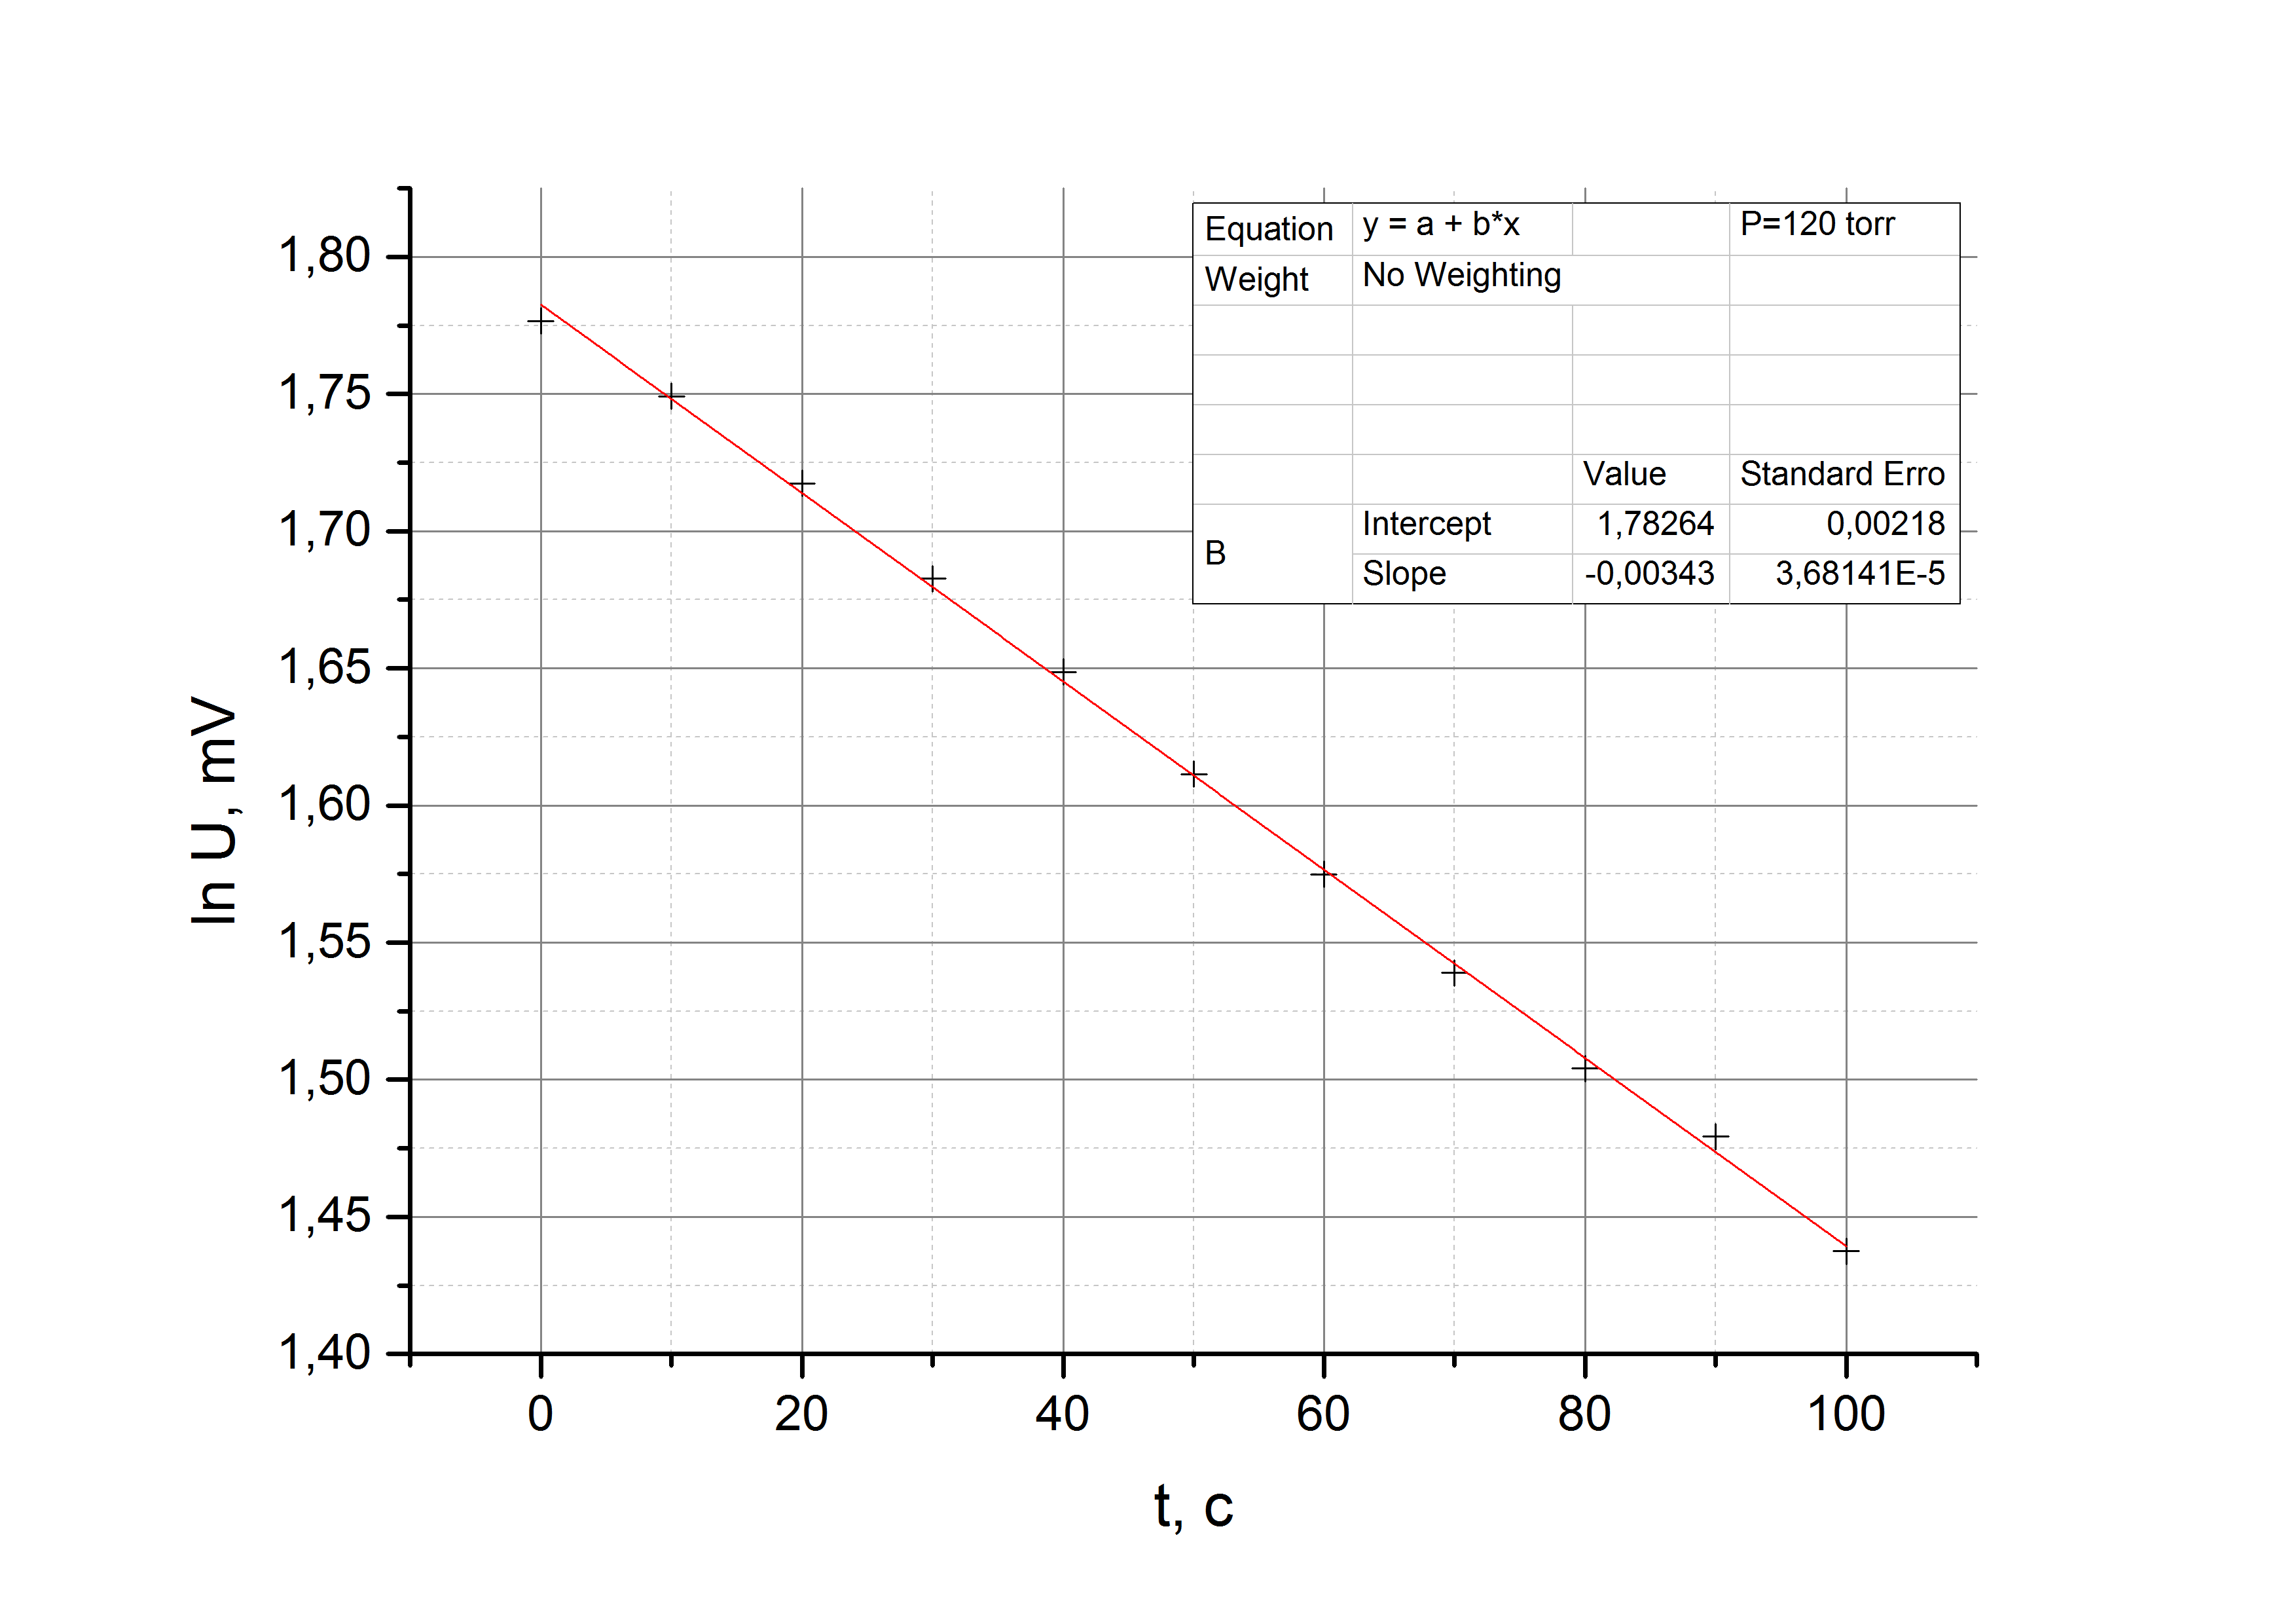
\includegraphics[width = 0.75\linewidth]{120torr}\newline
		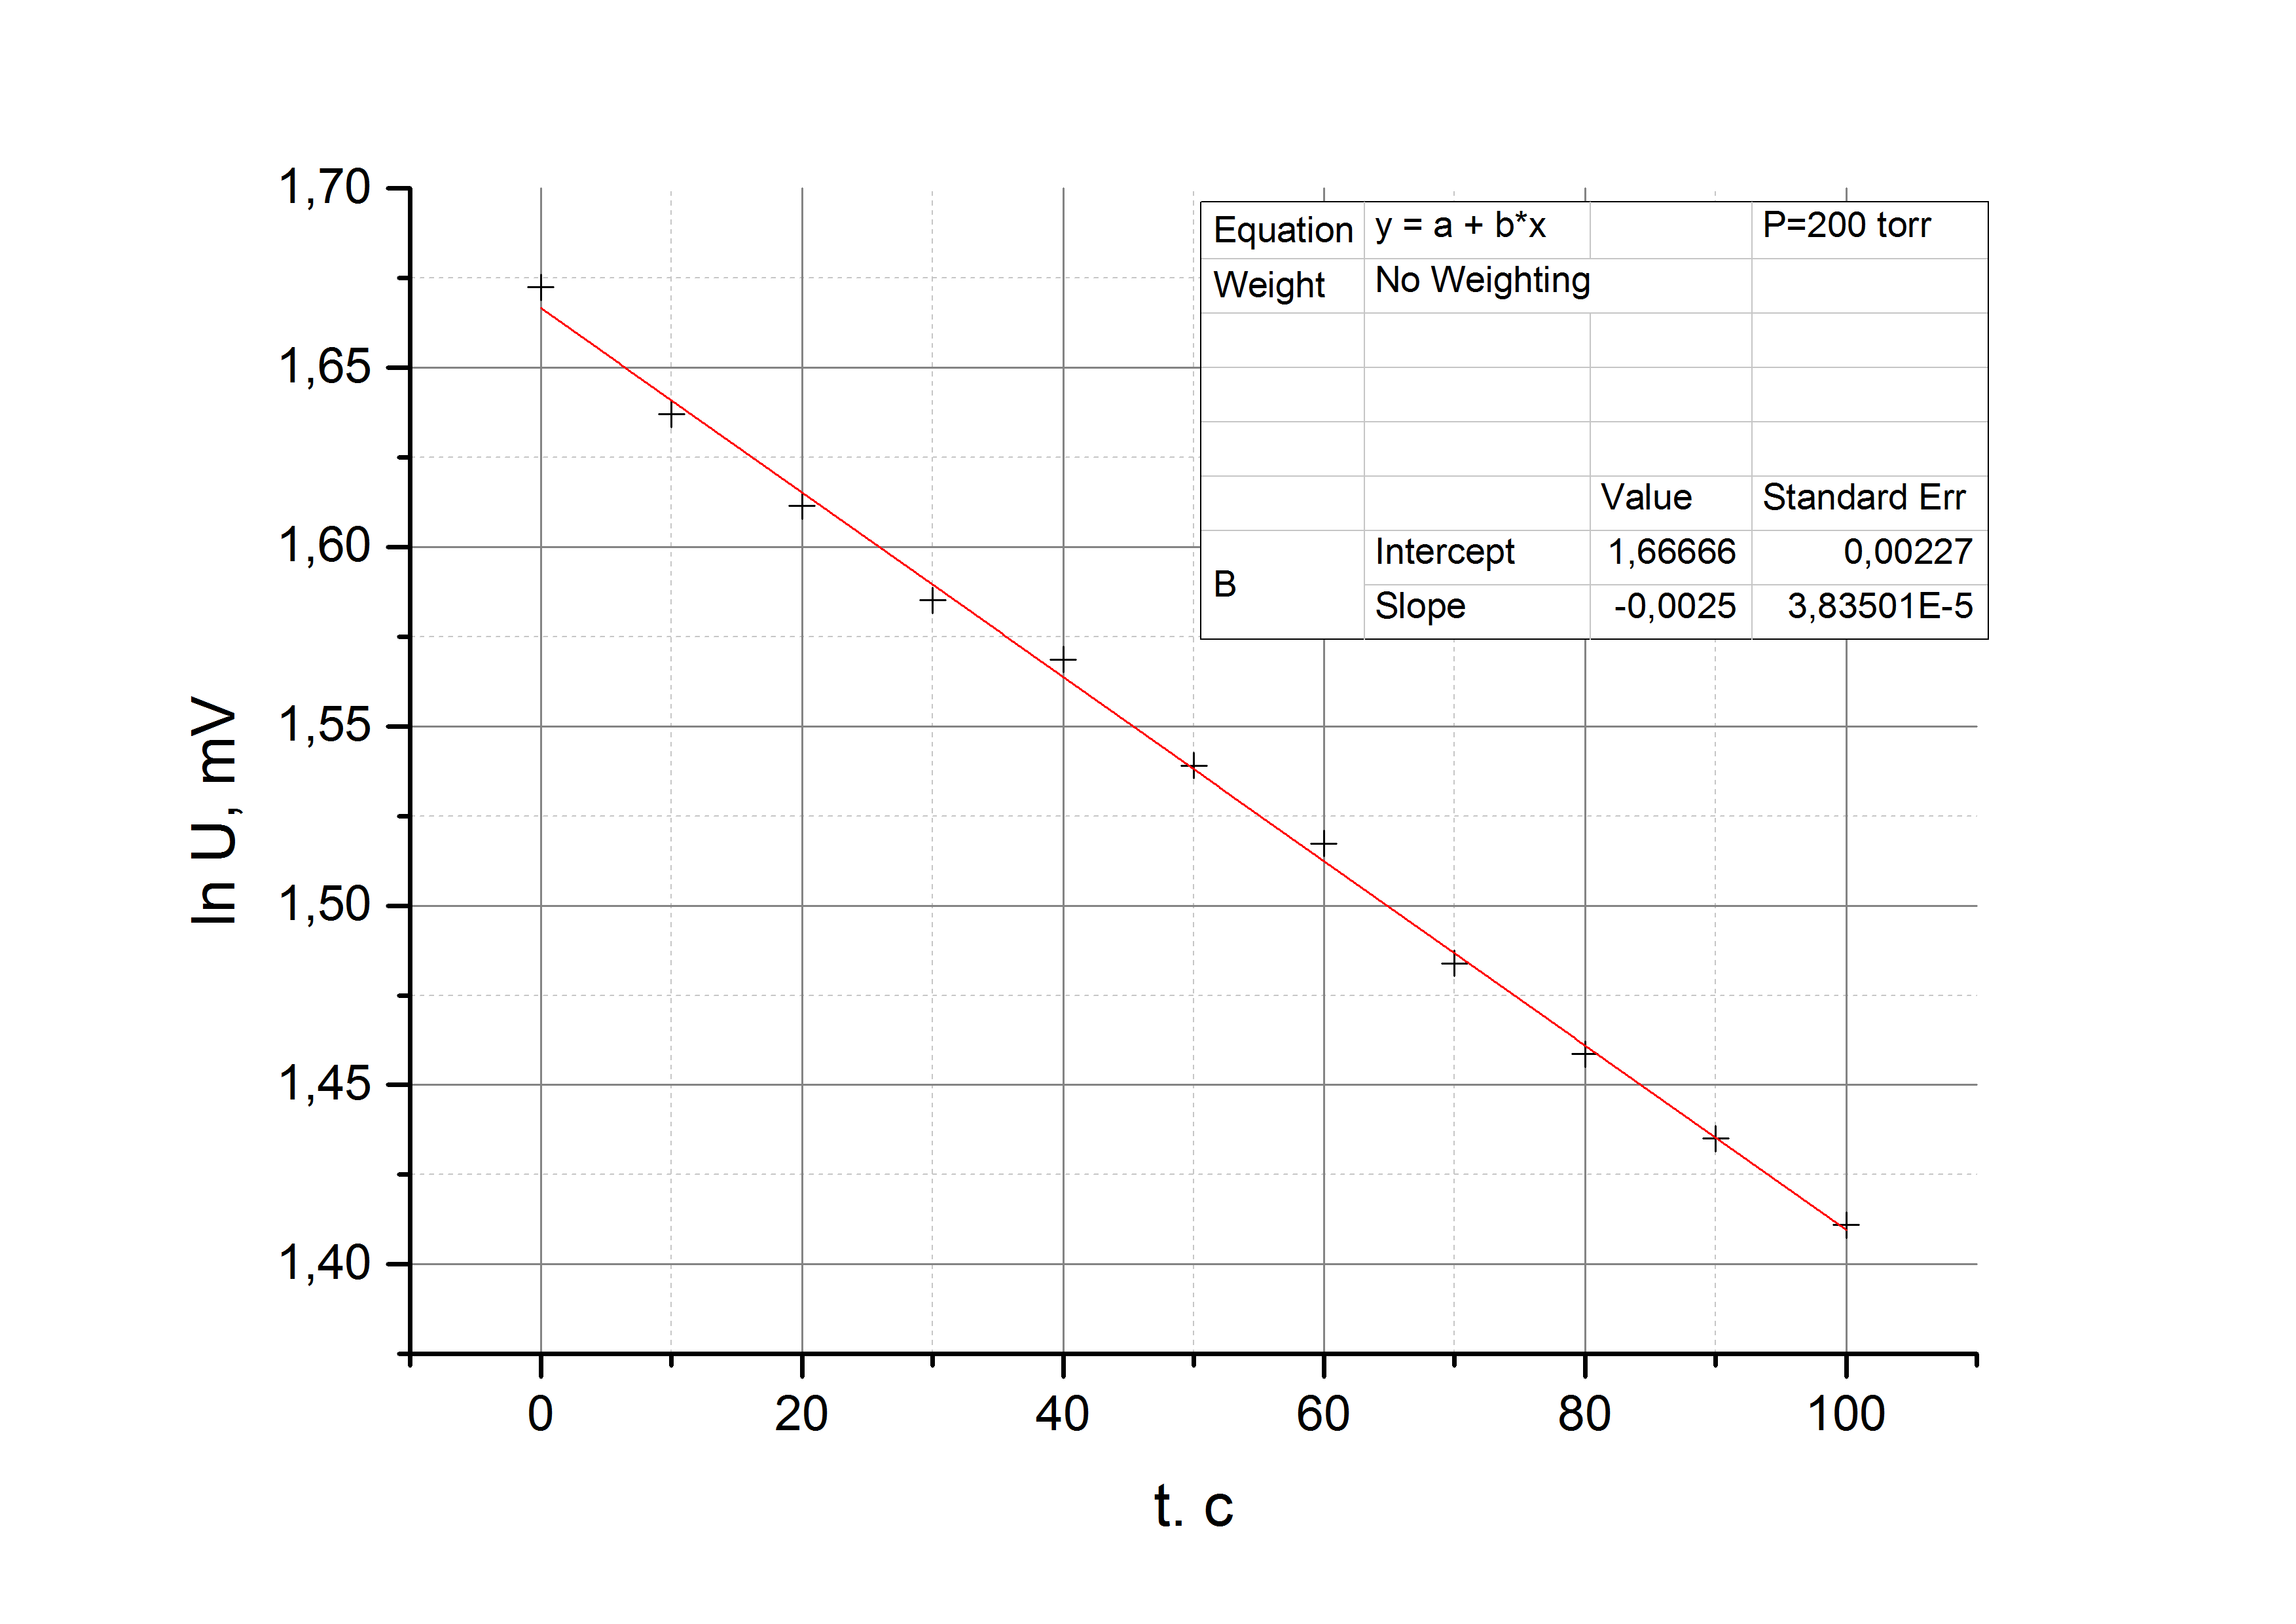
\includegraphics[width = 0.75\linewidth]{200torr}\newline
		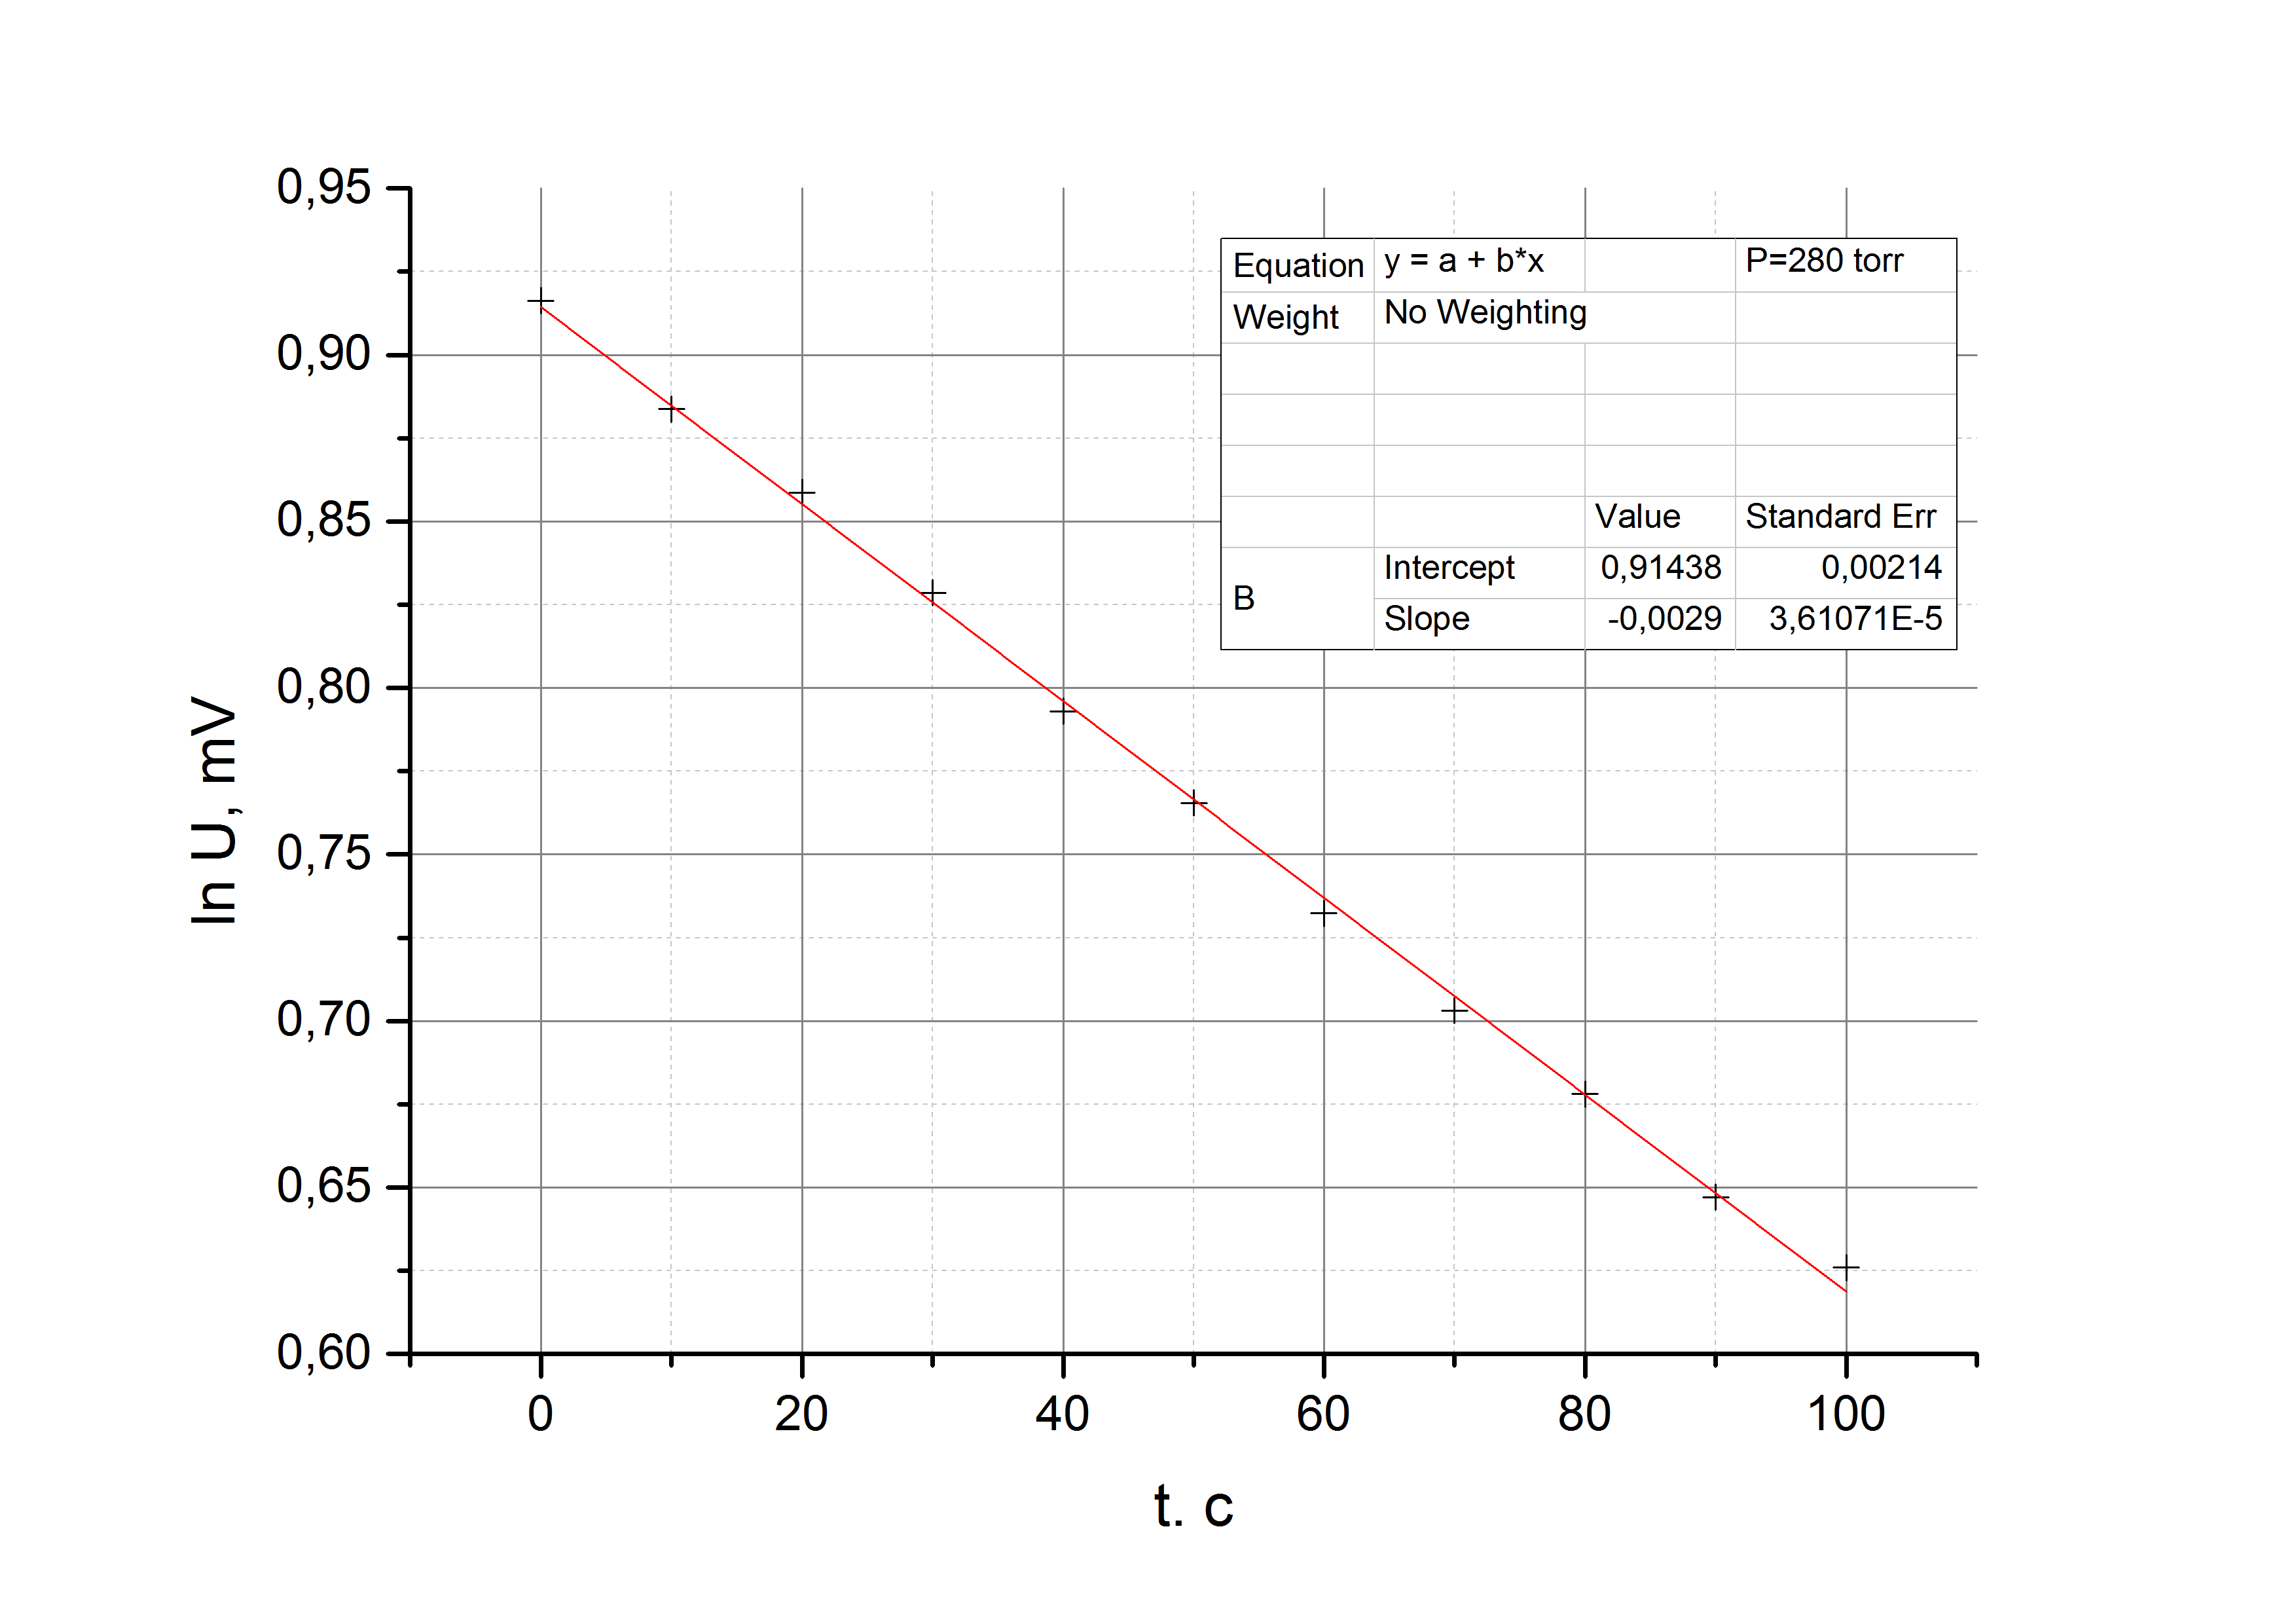
\includegraphics[width = 0.75\linewidth]{280torr}\newline
		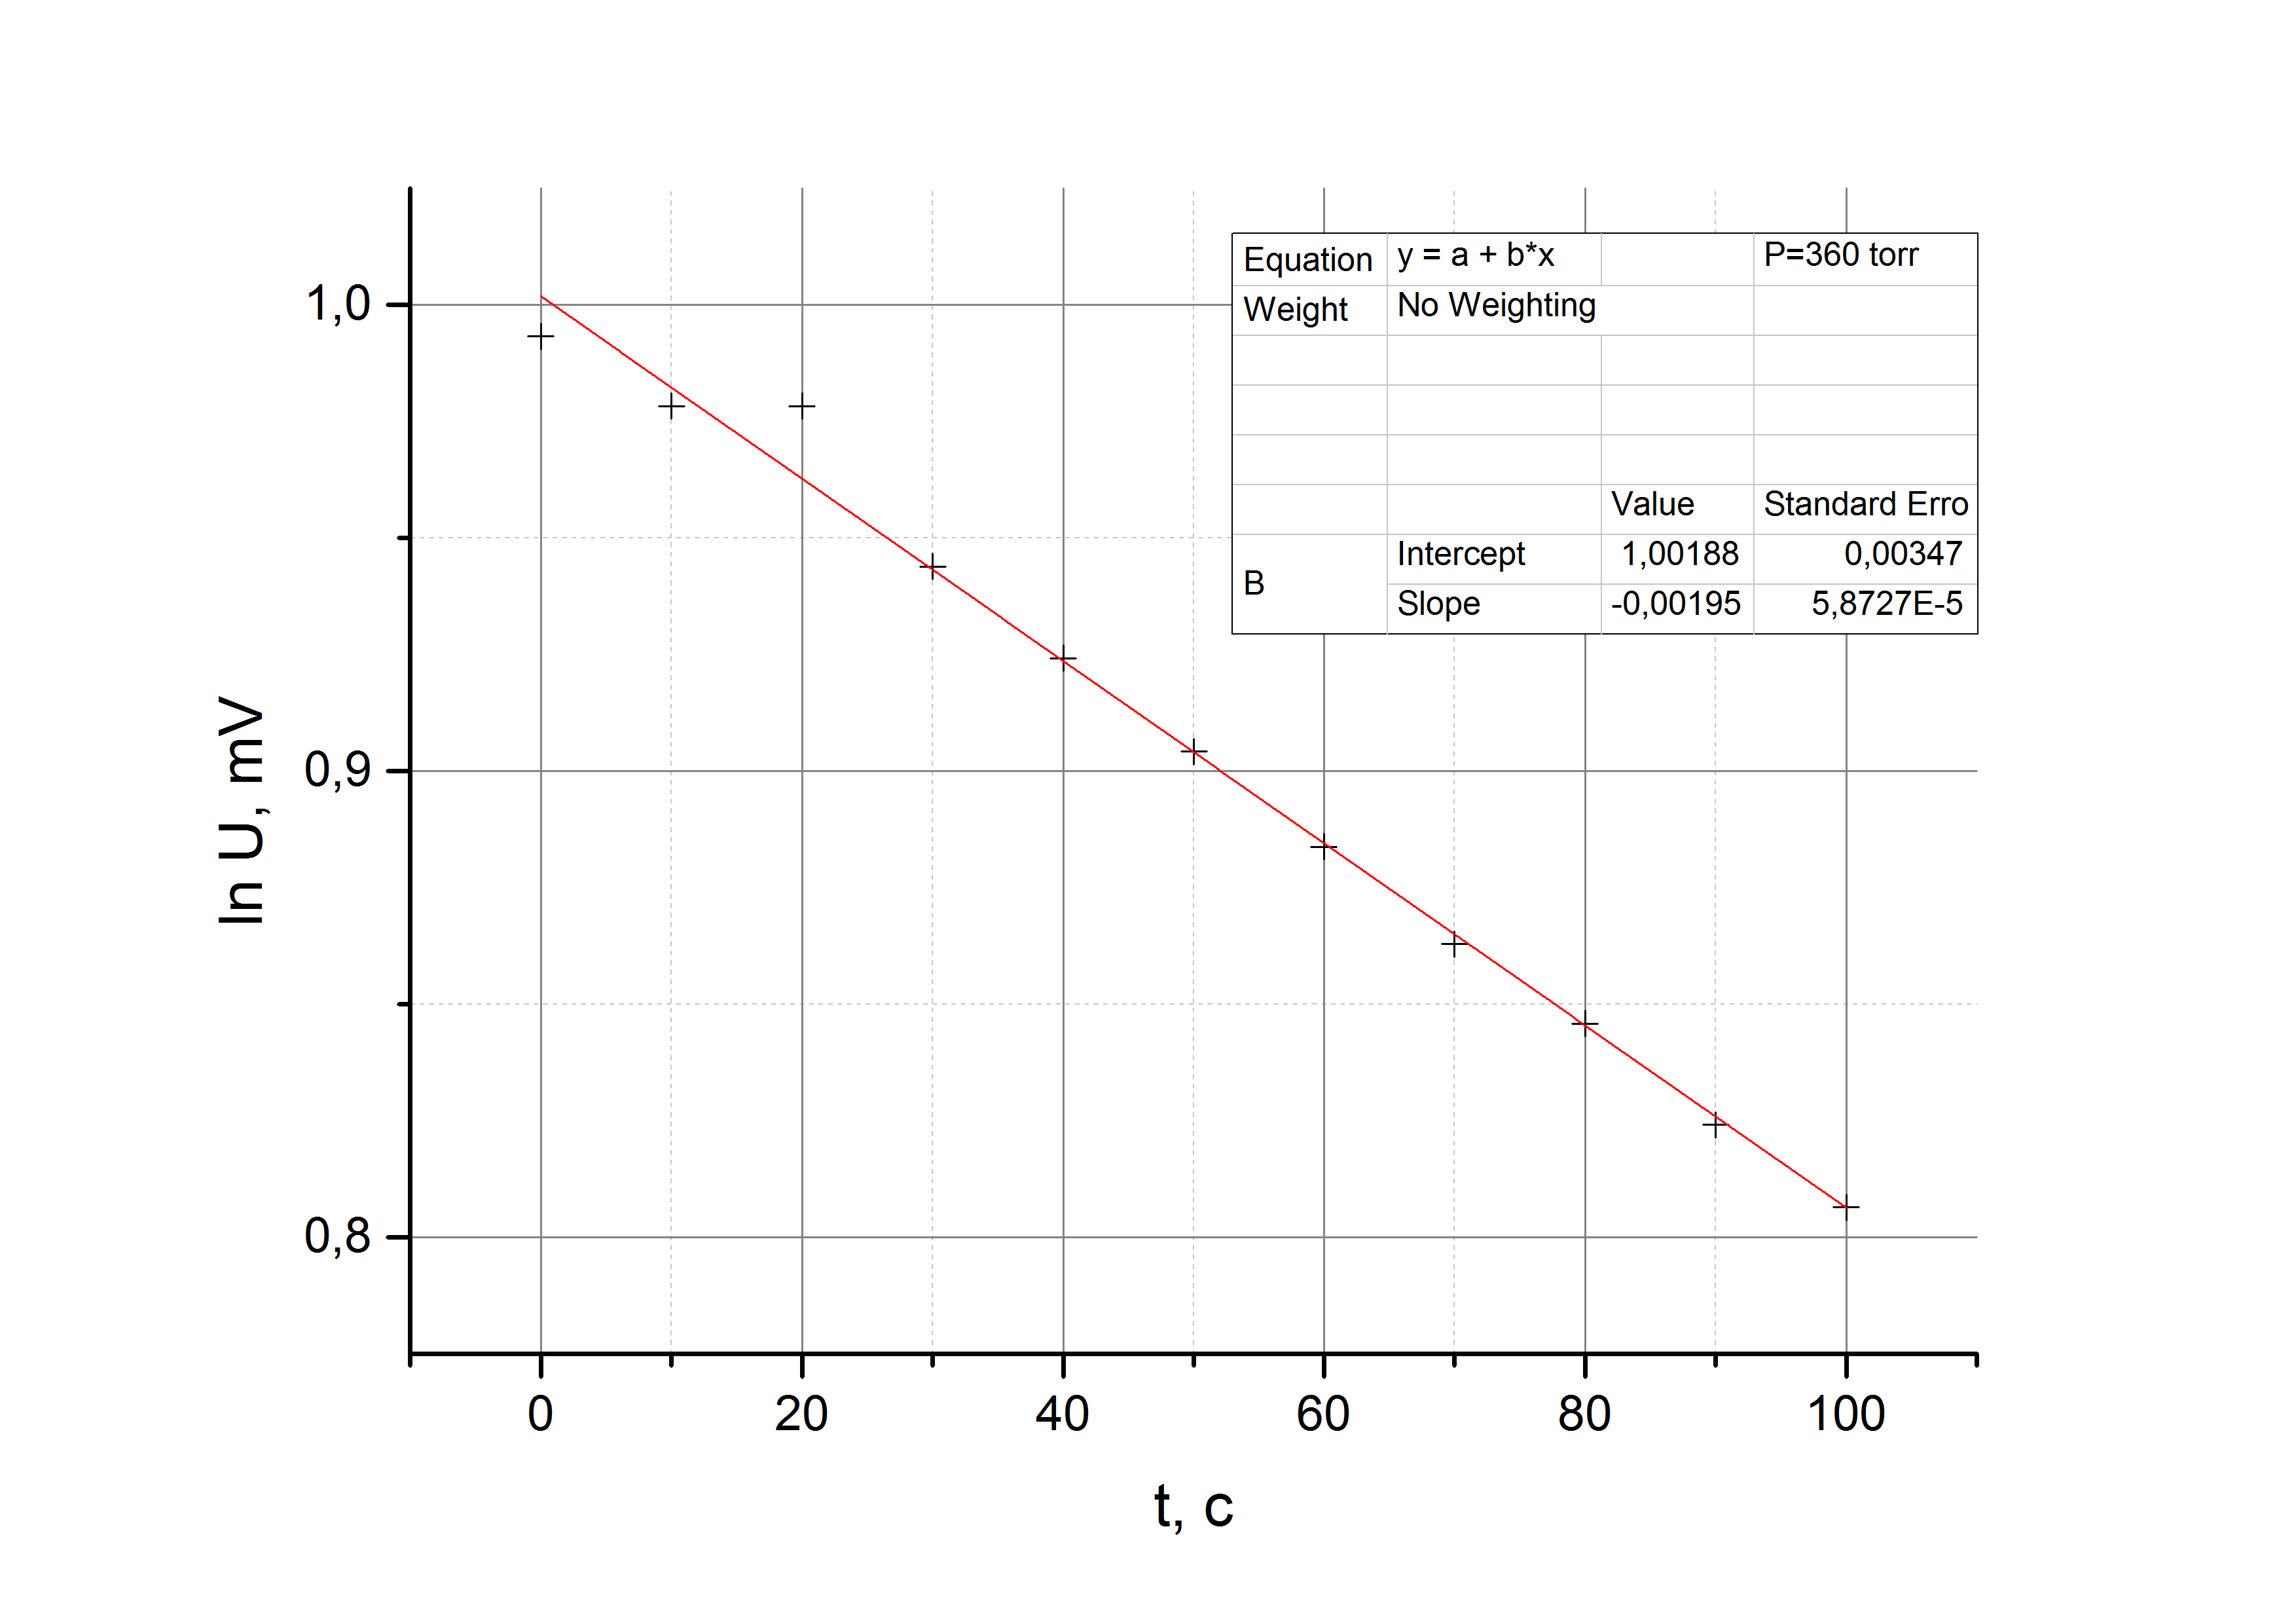
\includegraphics[width = 0.75\linewidth]{360torr}\newline

		По угловым коэффициентам графиков, используя равенство $D = \frac{a}{c}$ рассчитаем коэффициенты взаимных диффузий для разных давлений:
		\begin{center}
			\begin{tabular}{  l | l  p{1.5cm}  l  l  p{1.5cm}}
				P, торр                                & 40 & 120 & 200 & 280 & 360 \\ \hline
				$1/P$, торр$^{-1}$                     & 0.025 & 0.0083 & 0.005 & 0.0036 & 0.0028 \\ \hline
				$\sigma_{1/P}$,торр$^{-1}$             & 0.0062 & 0.002 & 0.00125 & 0.0009 & 0.0007 \\ \hline
				$\alpha\cdot 10^{-3}$, c$^{-1}$        & -7.2 & -3.4 & -2.5 & -2.9 & -1.95 \\ \hline
				$\sigma_{\alpha}\cdot 10^{-3}$, c$^{-1}$ & 0.7 & 0.12 & 0.1 & 0.1 & 0.11 \\ \hline
				$D$, м$^2\cdot$c$^{-1}$                & 0.36 & 0.17 & 0.125 & 0.145 &  0.01 \\ \hline
				$\sigma_D\cdot 10^{-3}$, м$^2\cdot$c$^{-1}$ & 5.04 & 2.38 & 1.75 & 2.03 & 1.4 \\ \hline
			\end{tabular}
		\end{center}
		
		Построим график $D(\frac{1}{P})$:
		
		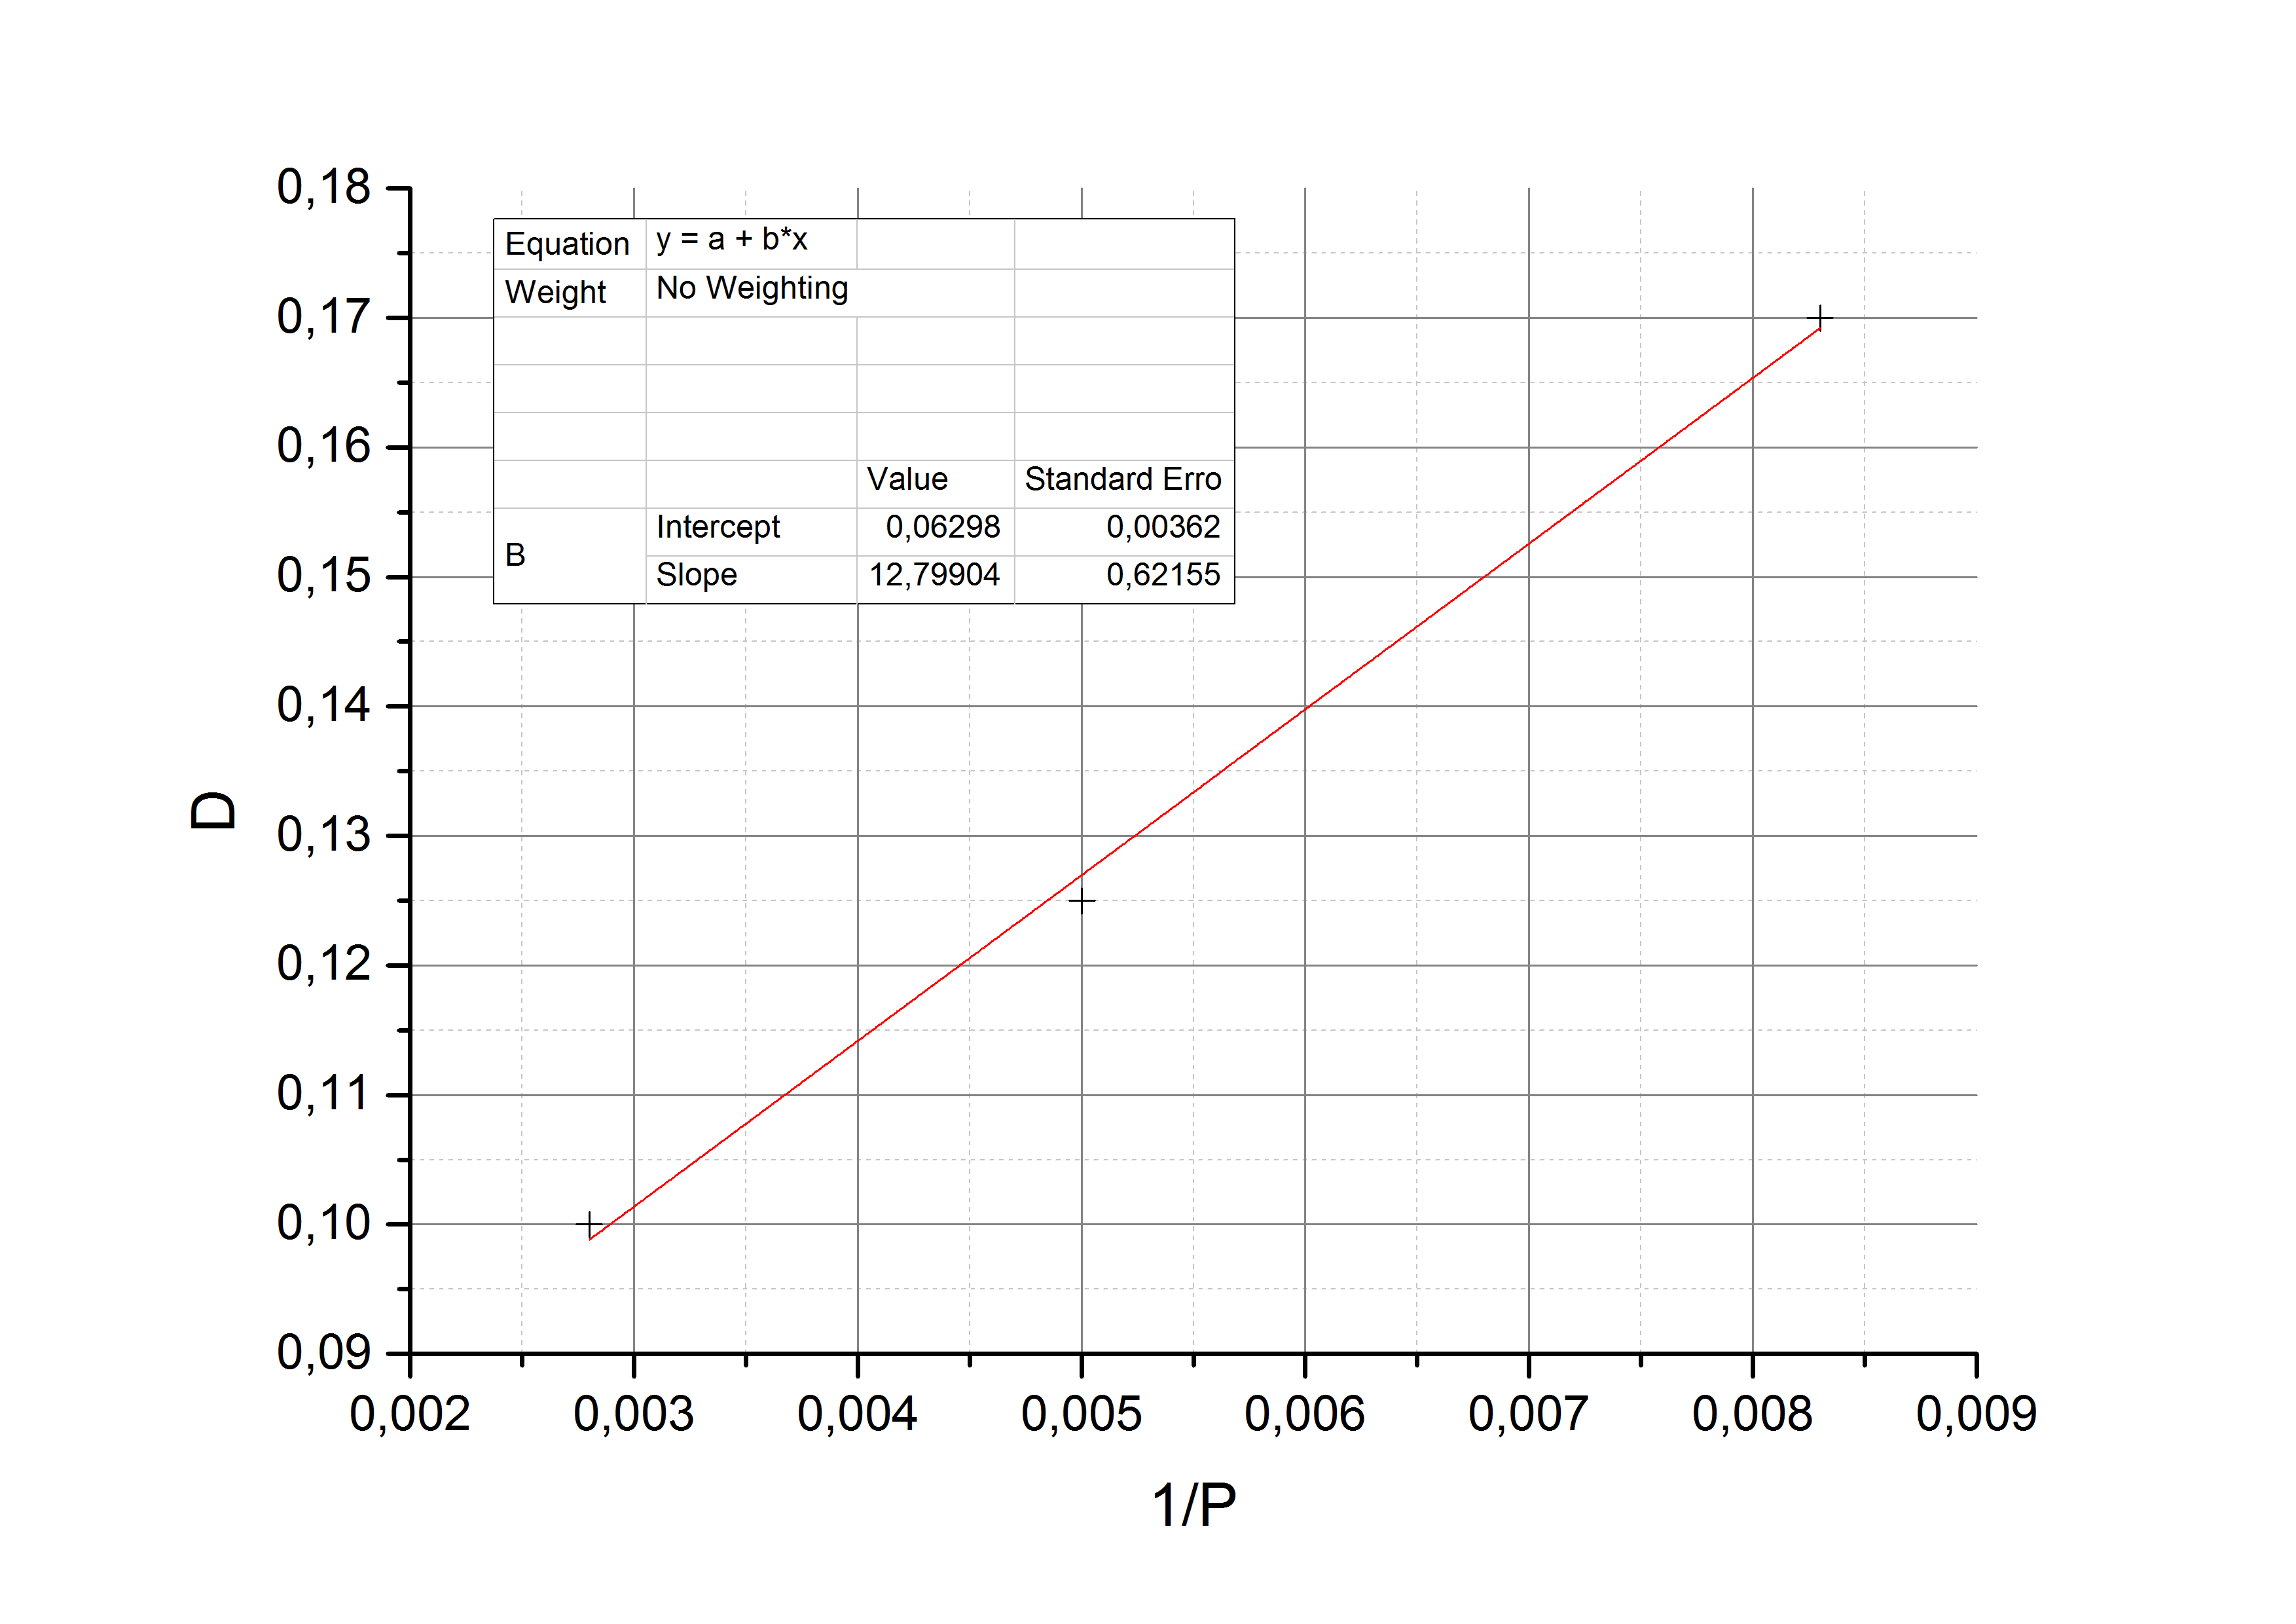
\includegraphics[width = 0.65\linewidth]{D}
		
		Апроксимируем полученную зависимость. Получим значение коэффициента -- диффузии при атмосферном давлении:
		\[
		D_{\text{атм}} = \left(0.79\pm 0.039\right)\frac{\text{см}^2}{\text{с}}
		\]
		Мы получили результат, близкий к табличному, с небольшой погрешностью.
		
		Оценим длину свободного пробега $\lambda$ и размер молекулы $d$:
		\[
		\lambda = 3D \sqrt{\frac{\mu}{3RT}} = \left(1.73 \pm 0.08\right)\cdot 10^{-7}\, \text{м}
		\]
		\[
		d = \sqrt{\frac{kT}{P\lambda}} \sim 6.4\cdot 10^{-11}
		\]
	\section{Вывод:}
		Измеряя данные о теплопроводности газов мы получили коэффициент взаимной диффузии, которых сходится с табличным по порядку, но немного расходится по значащей величине$ \left( D_{\text{табл}}=0.63 \,\frac{\text{см}^2}{\text{с}} \right)$. Из коэффициента взаимной дифуузии мы оценили длину свободного пробега молекулы гелия и её размер. Расхождение с табличными данными можно объяснить недостаточной точностью измерений и грубостью используемой модели о том, что концентрация воздуха практически не меняется.
\end{document}


